This chapter describes the design of our application, ... \todo{Other things than the application?}

The reader is expected to be familiar with standard Android components. Some components are briefly explained here:
\begin{description}
\item[Activity] An activity is a single focused thing that the user can do. You can also say that it is a window which is either full-screen or floating. \citep{activity}
\item[Fragment] A fragment inherits from activity and thus has its own lifecycle. Fragments are nested in activities, and can be used to build a multi-pane user interface. \citep{fragment}
\end{description}
\todo{Maybe add LinearLayout to the the list}

\section{Application Design}\label{sec:appdesign}

Before designing a prototype of our application we looked at a few other applications to get inspiration for our design.

\begin{figure}[H]
\begin{minipage}[b]{0.5\columnwidth}
\centering
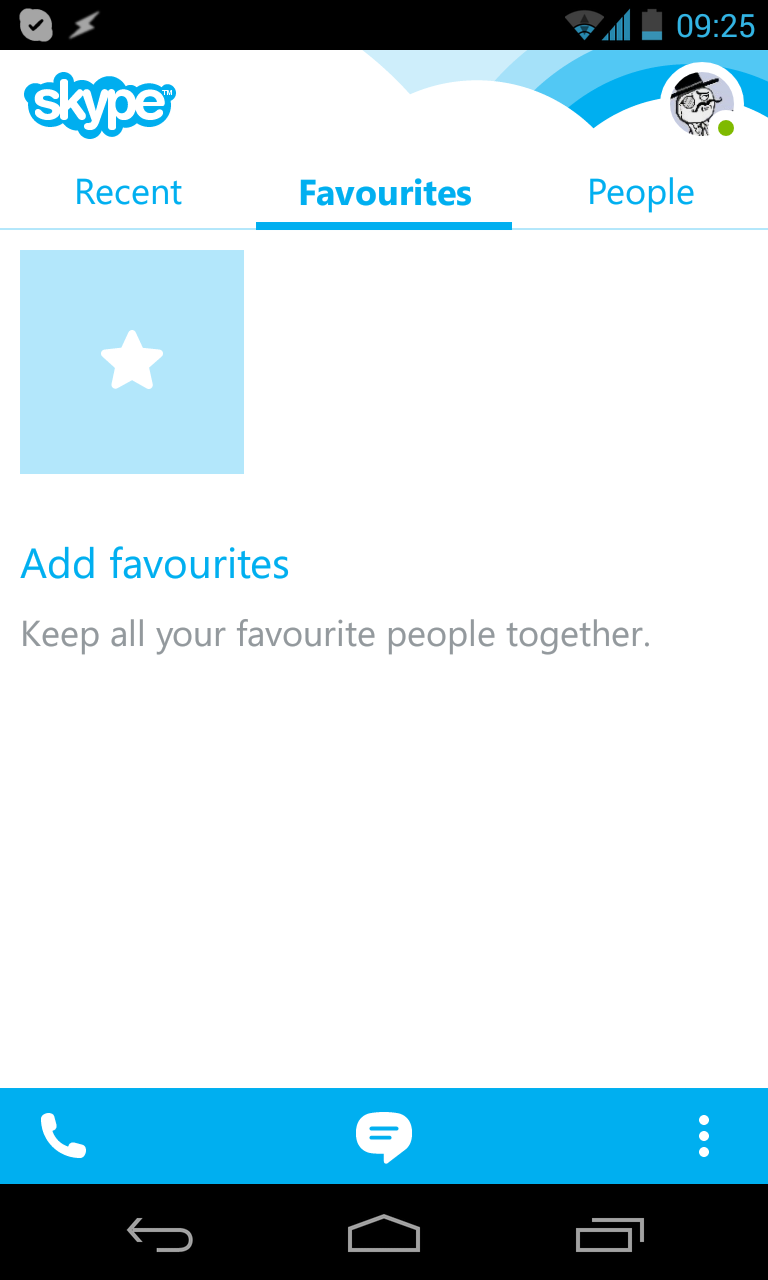
\includegraphics[width=0.7\columnwidth]{img/screenshots/twitter.png}
\caption{Skype\label{fig:skype}}
\end{minipage}
\hspace{0.5cm}
\begin{minipage}[b]{0.5\columnwidth}
\centering
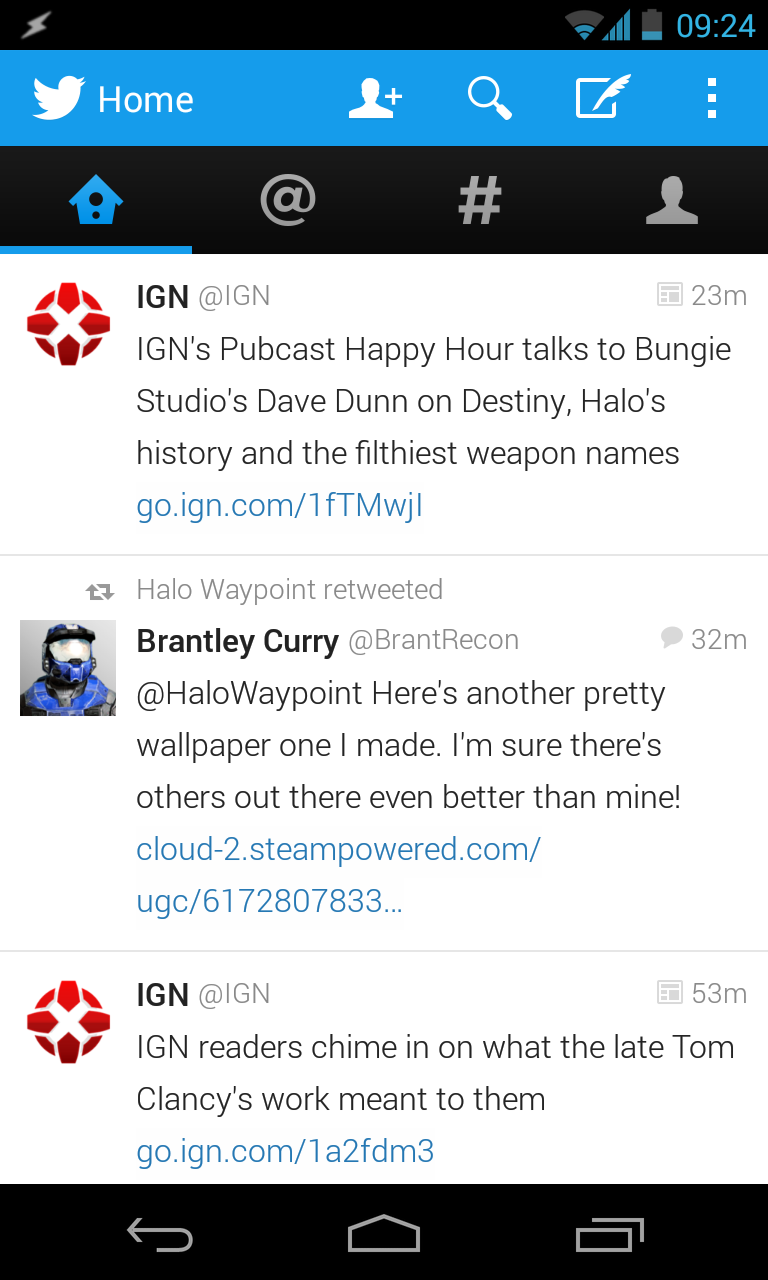
\includegraphics[width=0.7\columnwidth]{img/screenshots/skype.png}
\caption{Twitter\label{fig:twitter}}
\end{minipage}
\end{figure}

We decided that using tabs, like Skype in  \autoref{fig:skype}, was a good way for the user to easily see multiple pages of information by just swiping to the side.

We recognised that we were going to create a few different lists for the application e.g. a list of feeds and a schedule, for this we looked at Twitter \autoref{fig:twitter} and tried to capture their simplicity of tweets in our list items.

\subsection*{Story}
Julie opens our application Exhib. She is presented with a list of exhibitions that she browse. She browses the exhibitions and reads about them, she finds a software exhibition and decides that she want to go there. She clicks the map button which shows the exhibitions location. With her smartphone she can use her built-in \ac{gps} application to drive to the exhibition. When she arrives at the exhibition she quickly notices a sign that tells her to scan an \acs{nfc} tag. She scans the \acs{nfc} tag and the system registers a new user. An activity appears asking her what categories and related booths she would like to subscribe to. She picks Microsoft and clicks continue. Now she has access to everything about the exhibition: Exhibition information, map of the exhibition, news feed based on her subscriptions, and a schedule. Julie gets a quick overview of major events in the schedule and the news feed, and then decides to go directly to a Microsoft booth. On the map she finds a Microsoft booth, clicks it, and chose to get directions to the booth. The application remembers Julie's last known location, i.e. the last \acs{nfc} tag she scanned, and generates a route from there to the booth.

\section{Prototype Design}

Here we show our first revision of a prototype for our application. We created this together to reflect, visualise, and agree on the design.

\begin{figure}[H]
\begin{minipage}[b]{0.5\columnwidth}
\centering

\includegraphics[width=0.7\columnwidth]{img/prototype/1.png}
\caption{Start screen\label{fig:start}}
\end{minipage}
\hspace{0.5cm}
\begin{minipage}[b]{0.5\columnwidth}
\centering
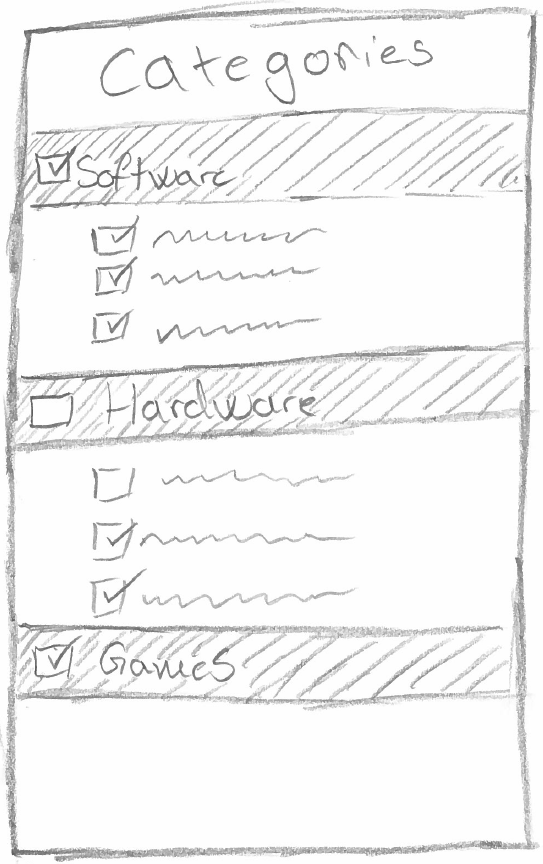
\includegraphics[width=0.7\columnwidth]{img/prototype/2.png}
\caption{Categories\label{fig:categories}}
\end{minipage}
\end{figure}

\autoref{fig:start} shows the application start screen. The user is told to scan an \ac{nfc} tag. When a tag is scanned the application checks if the user has visited the exhibition before. If the user has visited before then the exhibition information is opened, if not, then the user is asked to choose categories.

From the start screen you can also open a small menu in the bottom left corner where the user can browse for exhibitions and also pick recently visited exhibitions.

\autoref{fig:categories} is where you pick categories by clicking the check boxes. Although not present in the picture, the user should click submit in the bottom of the activity.

\begin{figure}[H]
\begin{minipage}[b]{0.5\columnwidth}
\centering
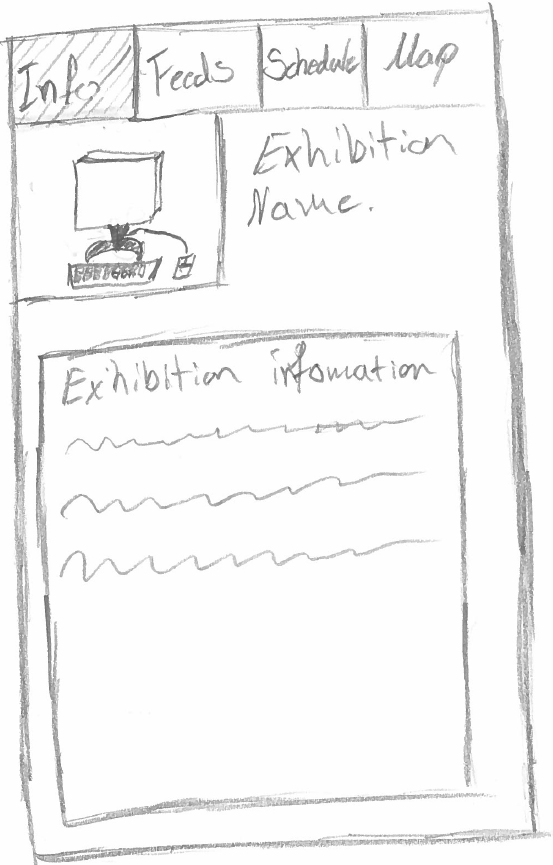
\includegraphics[width=0.7\columnwidth]{img/prototype/3.png}
\caption{Exhibition information\label{fig:exhibition}}
\end{minipage}
\hspace{0.5cm}
\begin{minipage}[b]{0.5\columnwidth}
\centering
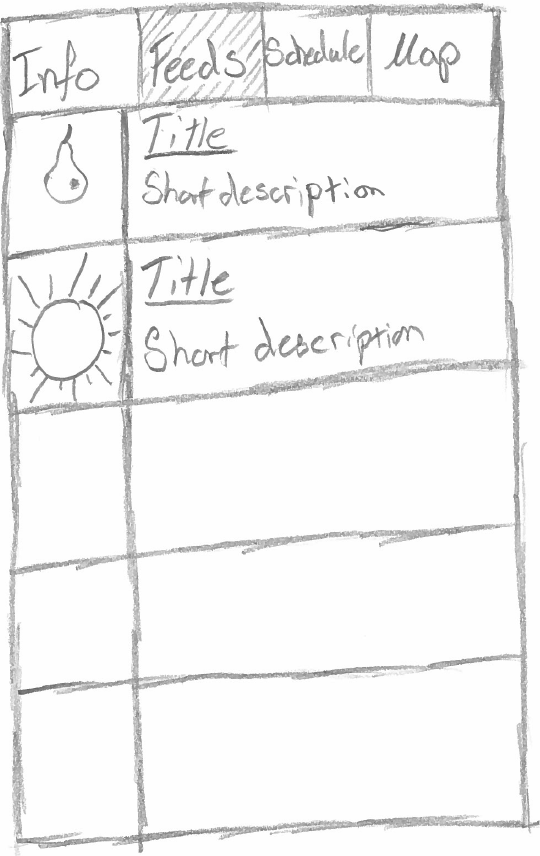
\includegraphics[width=0.7\columnwidth]{img/prototype/4.png}
\caption{Feed list\label{fig:feedlist}}
\end{minipage}
\end{figure}

When you are successfully registered at the exhibition, then you get to the core of the application. Here you can swipe between the different tabs, and also access a specific tab by clicking on it in the top menu. \autoref{fig:exhibition} shows the first tab, notice the tab bar in the top of the application showing which tab you are viewing. This is a simple welcome screen showing the exhibition icon, exhibition name, and an exhibition description.

\autoref{fig:feedlist} shows the feed list associated with the exhibition. The user receives feeds based on the chosen subscriptions that was submitted with the activity in \autoref{fig:categories}.

\begin{figure}[H]
\begin{minipage}[b]{0.5\columnwidth}
\centering
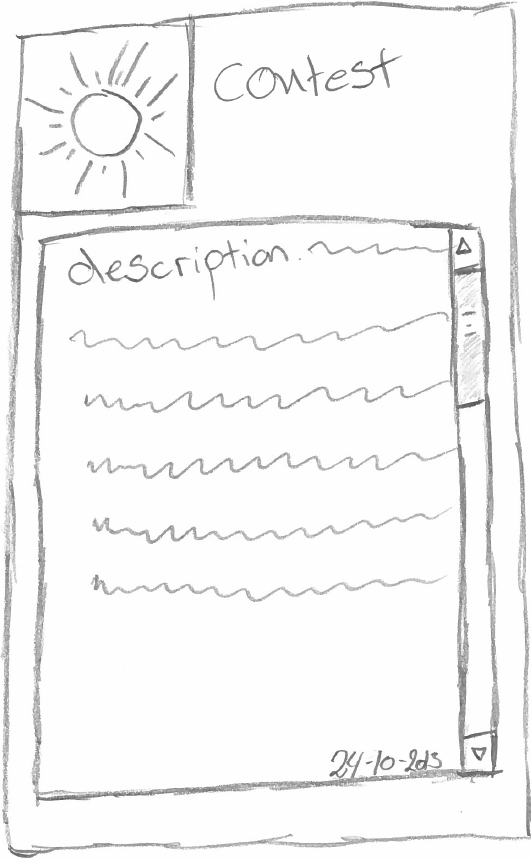
\includegraphics[width=0.7\columnwidth]{img/prototype/5.png}
\caption{Feed item\label{fig:feeditem}}
\end{minipage}
\hspace{0.5cm}
\begin{minipage}[b]{0.5\columnwidth}
\centering
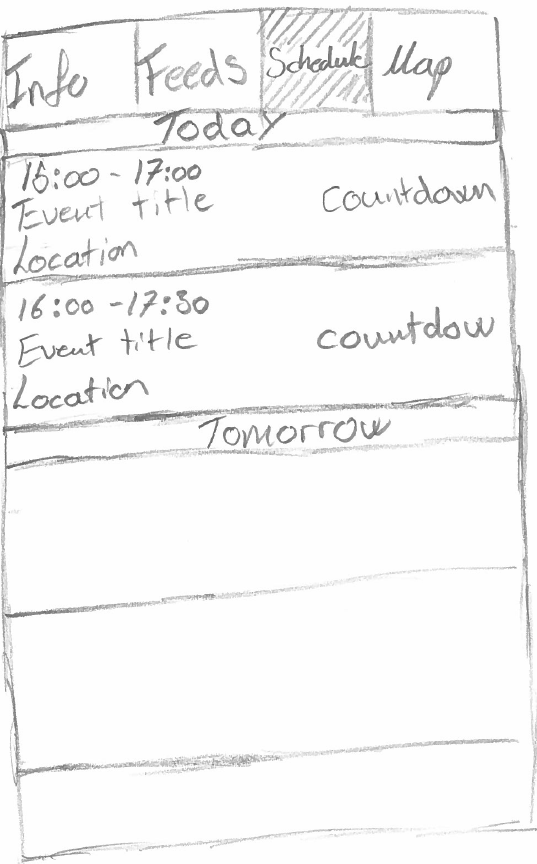
\includegraphics[width=0.7\columnwidth]{img/prototype/6.png}
\caption{Schedule\label{fig:schedule}}
\end{minipage}
\end{figure}

\autoref{fig:feeditem} is the activity shown when you click a feed item from the feed list. A feed item consists of a headline, a feed description, and it shows the icon attached to the booth which is associated with the feed item.

\autoref{fig:schedule} shows the schedule of the exhibition. The schedule items are grouped by days. Each schedule item shows the time interval of the event, a title, a location, and it shows a continuously updated countdown to the event.

\begin{figure}[H]
\begin{minipage}[b]{0.5\columnwidth}
\centering
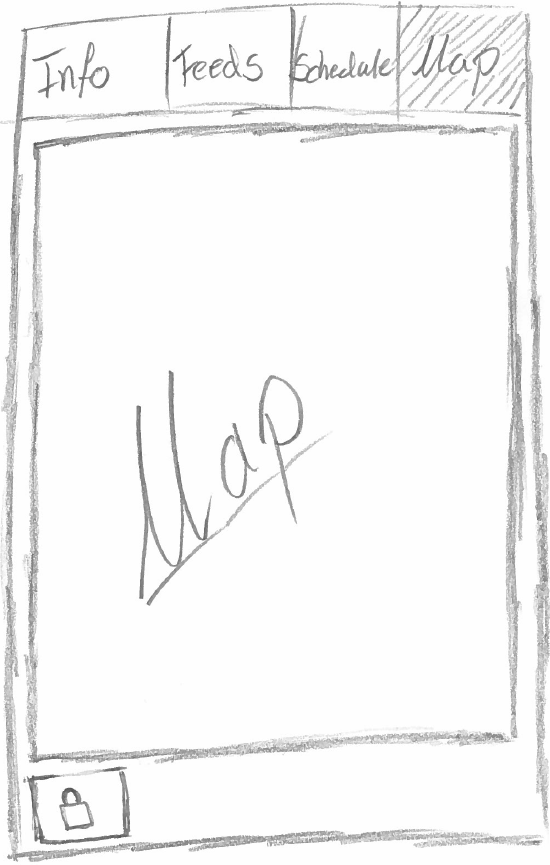
\includegraphics[width=0.7\columnwidth]{img/prototype/7.png}
\caption{Map\label{fig:map}}
\end{minipage}
\hspace{0.5cm}
\begin{minipage}[b]{0.5\columnwidth}
\centering
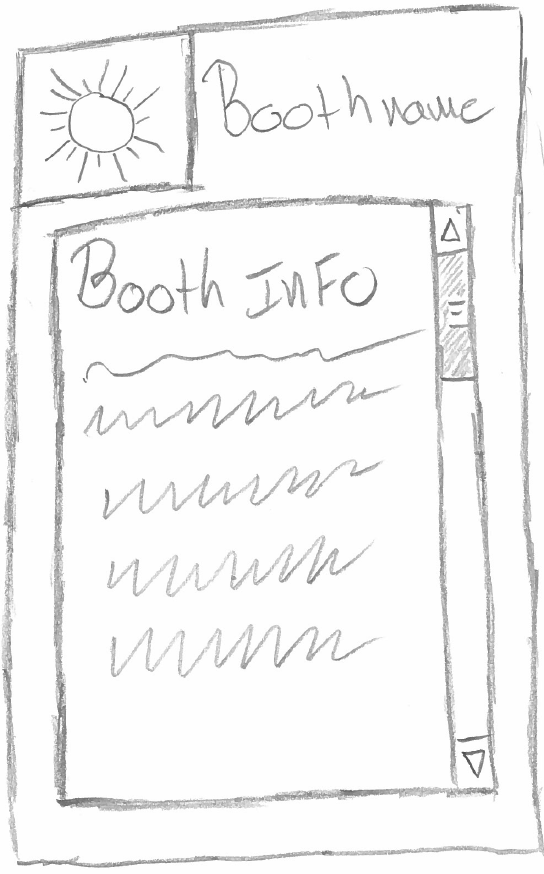
\includegraphics[width=0.7\columnwidth]{img/prototype/8.png}
\caption{Booth information\label{fig:booth}}
\end{minipage}
\end{figure}

\autoref{fig:map} shows the tab displaying the map of the exhibition. Below the map there is a lock button, which locks the user to navigating the map e.g. swiping left and right on the map. If it is not locked then swiping right will change to the schedule tab. Inside the map there should be pinned booths which can be clicked on. When clicking the booths the activity shown in \autoref{fig:booth} is opened. The booth activity shows its attached icon, a name, and information concerning the booth.

\section{Final Application Design}

The final application consists of the following activities and fragments:

\begin{description}
\item[MainActivity] This is the startup activity. This activity waits for the user to scan an \ac{nfc} tag and redirect the user appropriately.
\item[TabActivity] The core of the application, contains all the tabs i.e. fragments.
\item[ExhibitionInformationFragment] Shows information about an exhibition such as name, description, and logo.
\item[FloorplanFragment] Shows the map of the exhibition. The map contains markers for each booth which the user can click to access information about the booth.
\item[ScheduleFragment] Is a schedule for the exhibition which shows major events happening at the exhibition.
\item[FeedFragment] Is a list of news feeds based on the users subscriptions.
\item[FeedActivity] Shows the feed item when it is clicked from the feed list.
\item[CategoriesActivity] Is a list of categories, e.g. hardware, software.
\end{description}
We did not create the \textit{BoothActivity} which is showed in \autoref{fig:booth}, because we realised that we might as well show all the booth information in the marker information window on the map. This is shown later in this section.

\section*{Final design}
The following section shows our final design of our application. A run-through of each of the screen that you may encounter throughout the application.

When opening the application the first screen you encouter is one telling the user to scan an \ac{nfc} tag. The screen is shown on \autoref{fig:nfcscreen}. The windows differs from the protoype, as there is no menu in the bottom right to browse exhibitions. When the \ac{nfc} tag is scanned you are signed up to that specific exhibition and a new screen appears asking the user to choose between different categories and booths, this is to identify the users interests which will be used later by the application. This is shown on \autoref{fig:categories1}. After the user has selected their categories, they press submit. Note that after having scanned and chosen categories the first time, the next time the user opens the application and scan an \ac{nfc} tag from the same exhibition, the user does not have to choose categories and booths again.

\begin{figure}[H]
\begin{minipage}[b]{0.5\columnwidth}
\centering
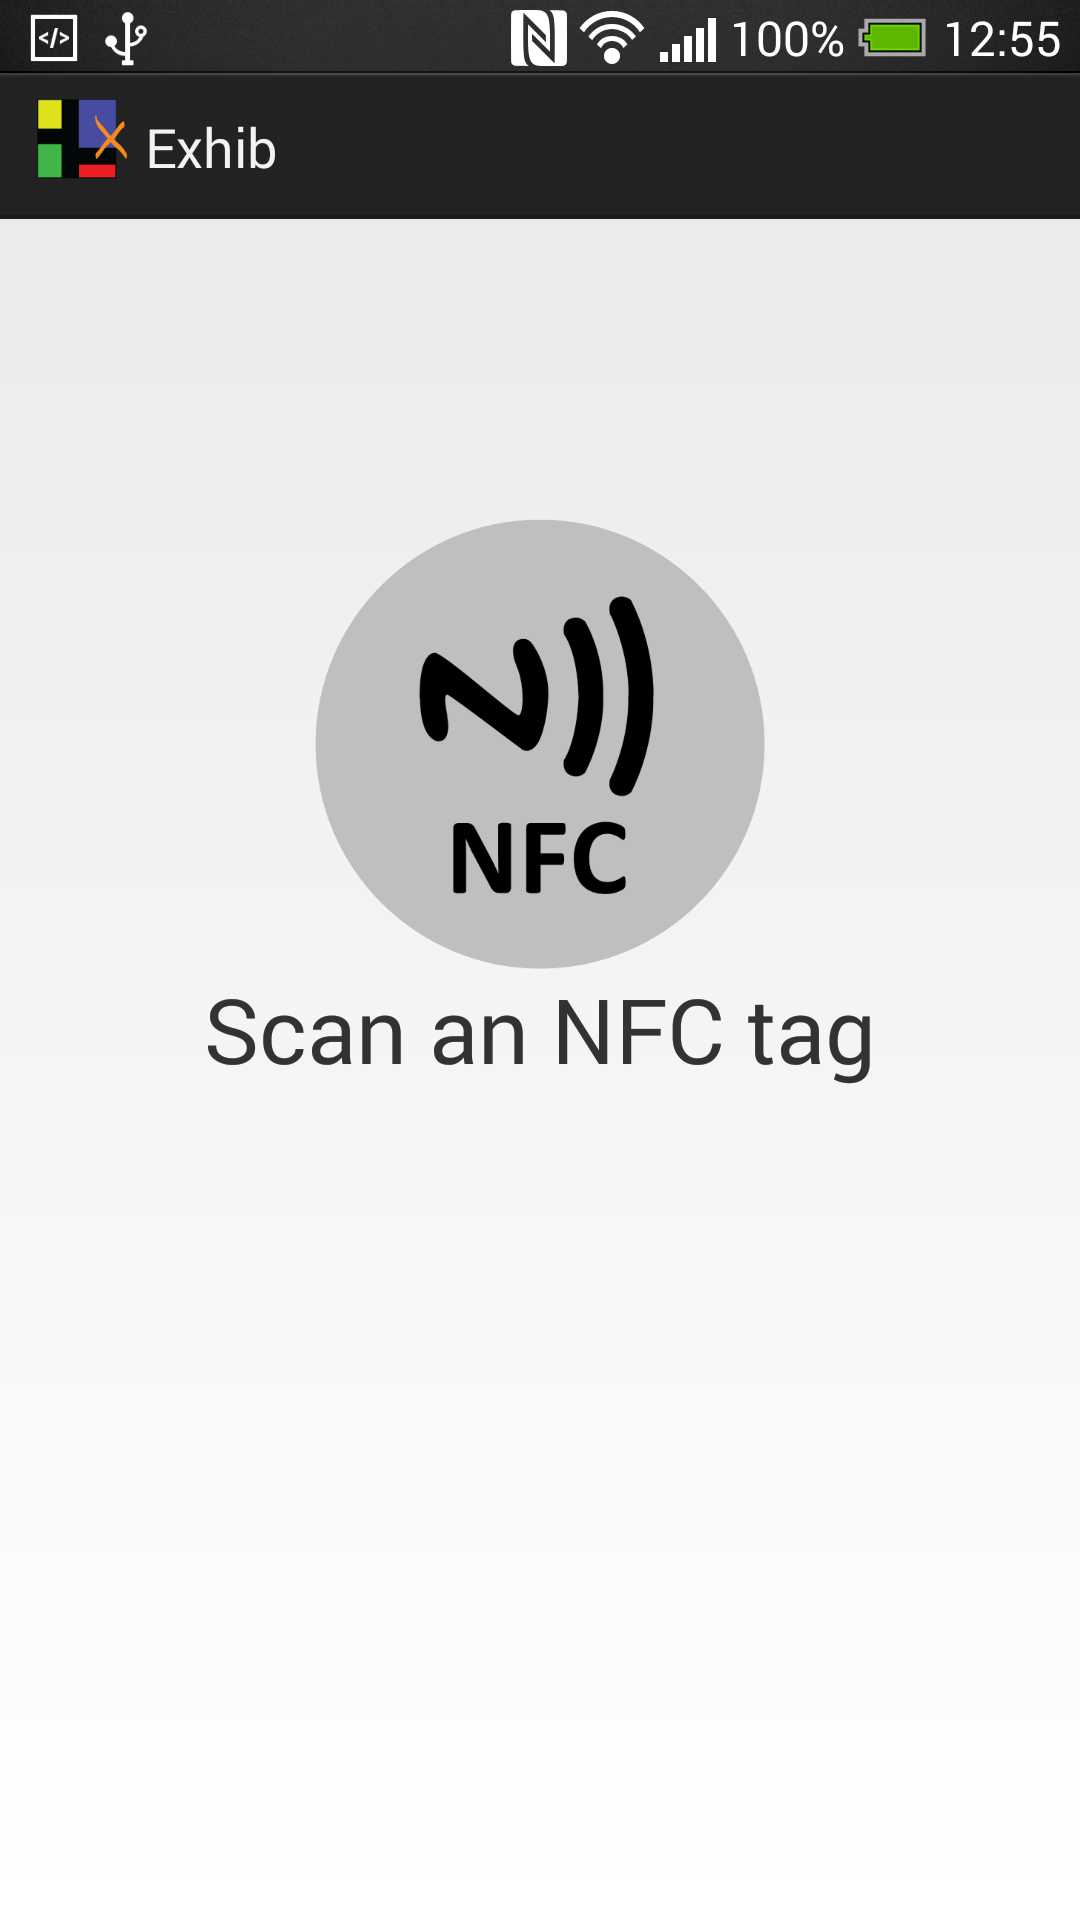
\includegraphics[width=0.7\columnwidth]{img/finaldesign/nfcscreen.png}
\caption{Start screen}
\label{fig:nfcscreen}
\end{minipage}
\hspace{0.5cm}
\begin{minipage}[b]{0.5\columnwidth}
\centering
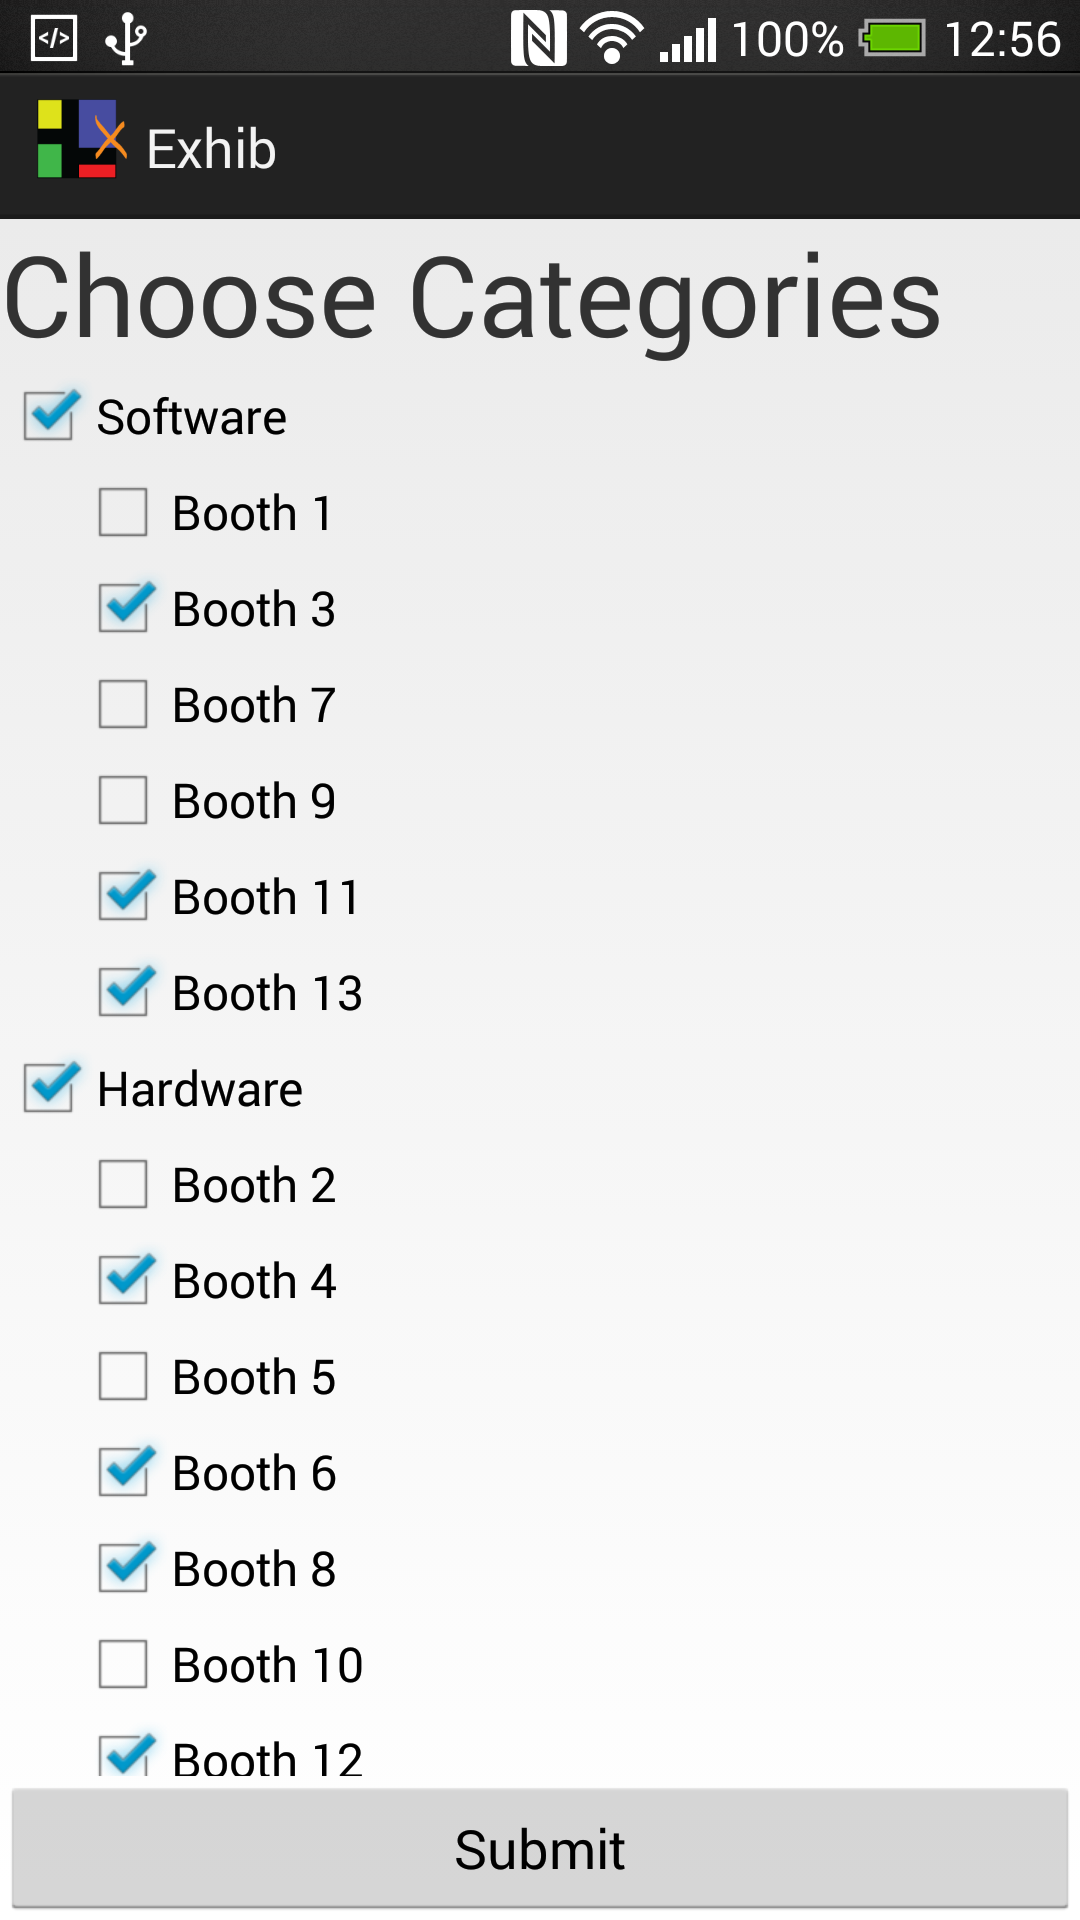
\includegraphics[width=0.7\columnwidth]{img/finaldesign/categories.png}
\caption{Categories}
\label{fig:categories1}
\end{minipage}
\end{figure}

After having submitted the categories the user want to subscribe to, the user will be taken to an "Info" tab, this is a simple tab displaying information about exhibition the user are currently at, such as exhibition logo, name and a description of the exhibition. This can be seen on \autoref{fig:infoscreen}  at the top. Next to "Info" there are three other tabs: "Feeds", "Schedule", and "Map". These four tabs can be navigated to and from, from any of the other tabs either by swiping from side to side or by clicking on the tab itself at the top.

The tab "Feeds", as seen on\autoref{fig:feedsscreen}, shows a list feeds made by booths at the exhibition. The application uses the booths that the user subscribed to before, the user only receives feeds from the booths that they subscribed to after scanning the \ac{nfc} tag. Each feed has a timestamp telling the user when it was made.

It is also possible for the user to change the booths they have subscribed to, if they want to receive different feeds. This is done by pressing the three vertical dots in the top right corner, this takes they user to the categories screen again where they can choose new categories and booths. 

\begin{figure}[H]
\begin{minipage}[b]{0.5\columnwidth}
\centering
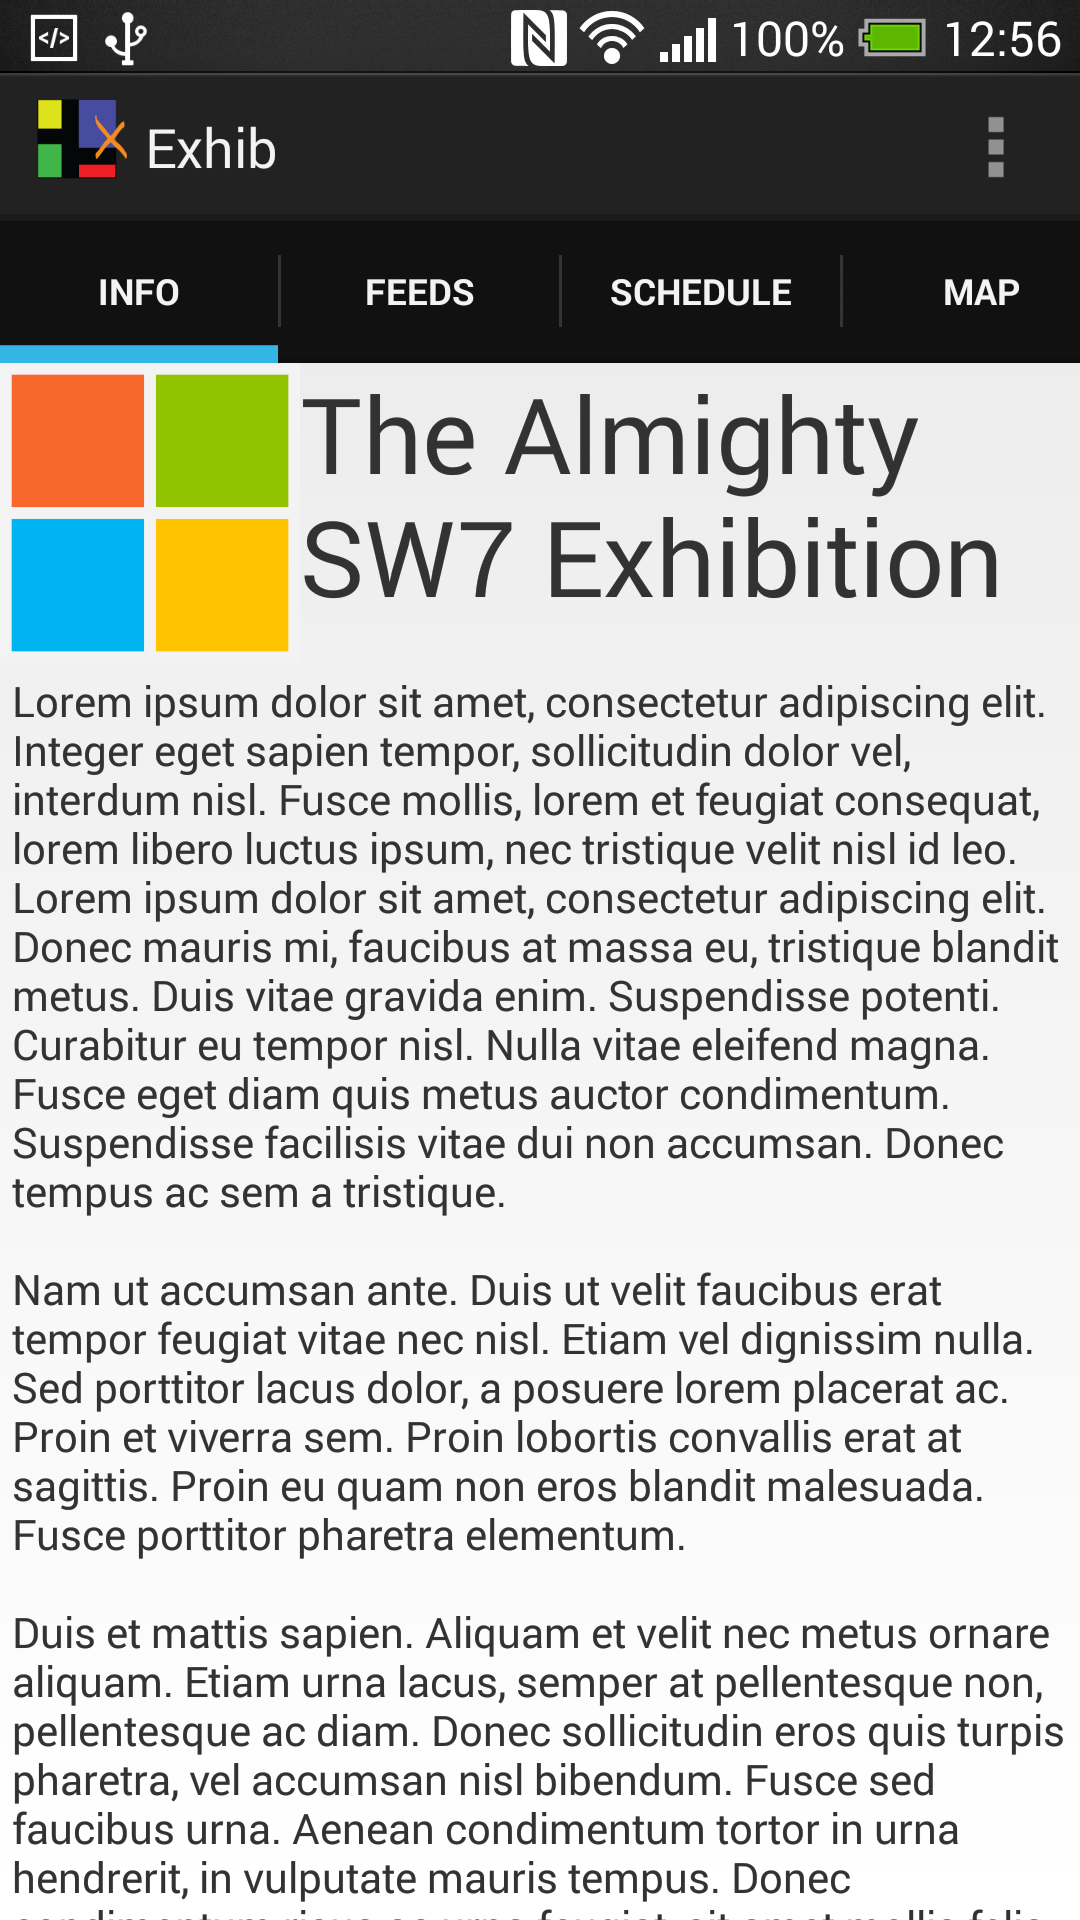
\includegraphics[width=0.7\columnwidth]{img/finaldesign/infoscreen.png}
\caption{Exhibition information}
\label{fig:infoscreen}
\end{minipage}
\hspace{0.5cm}
\begin{minipage}[b]{0.5\columnwidth}
\centering
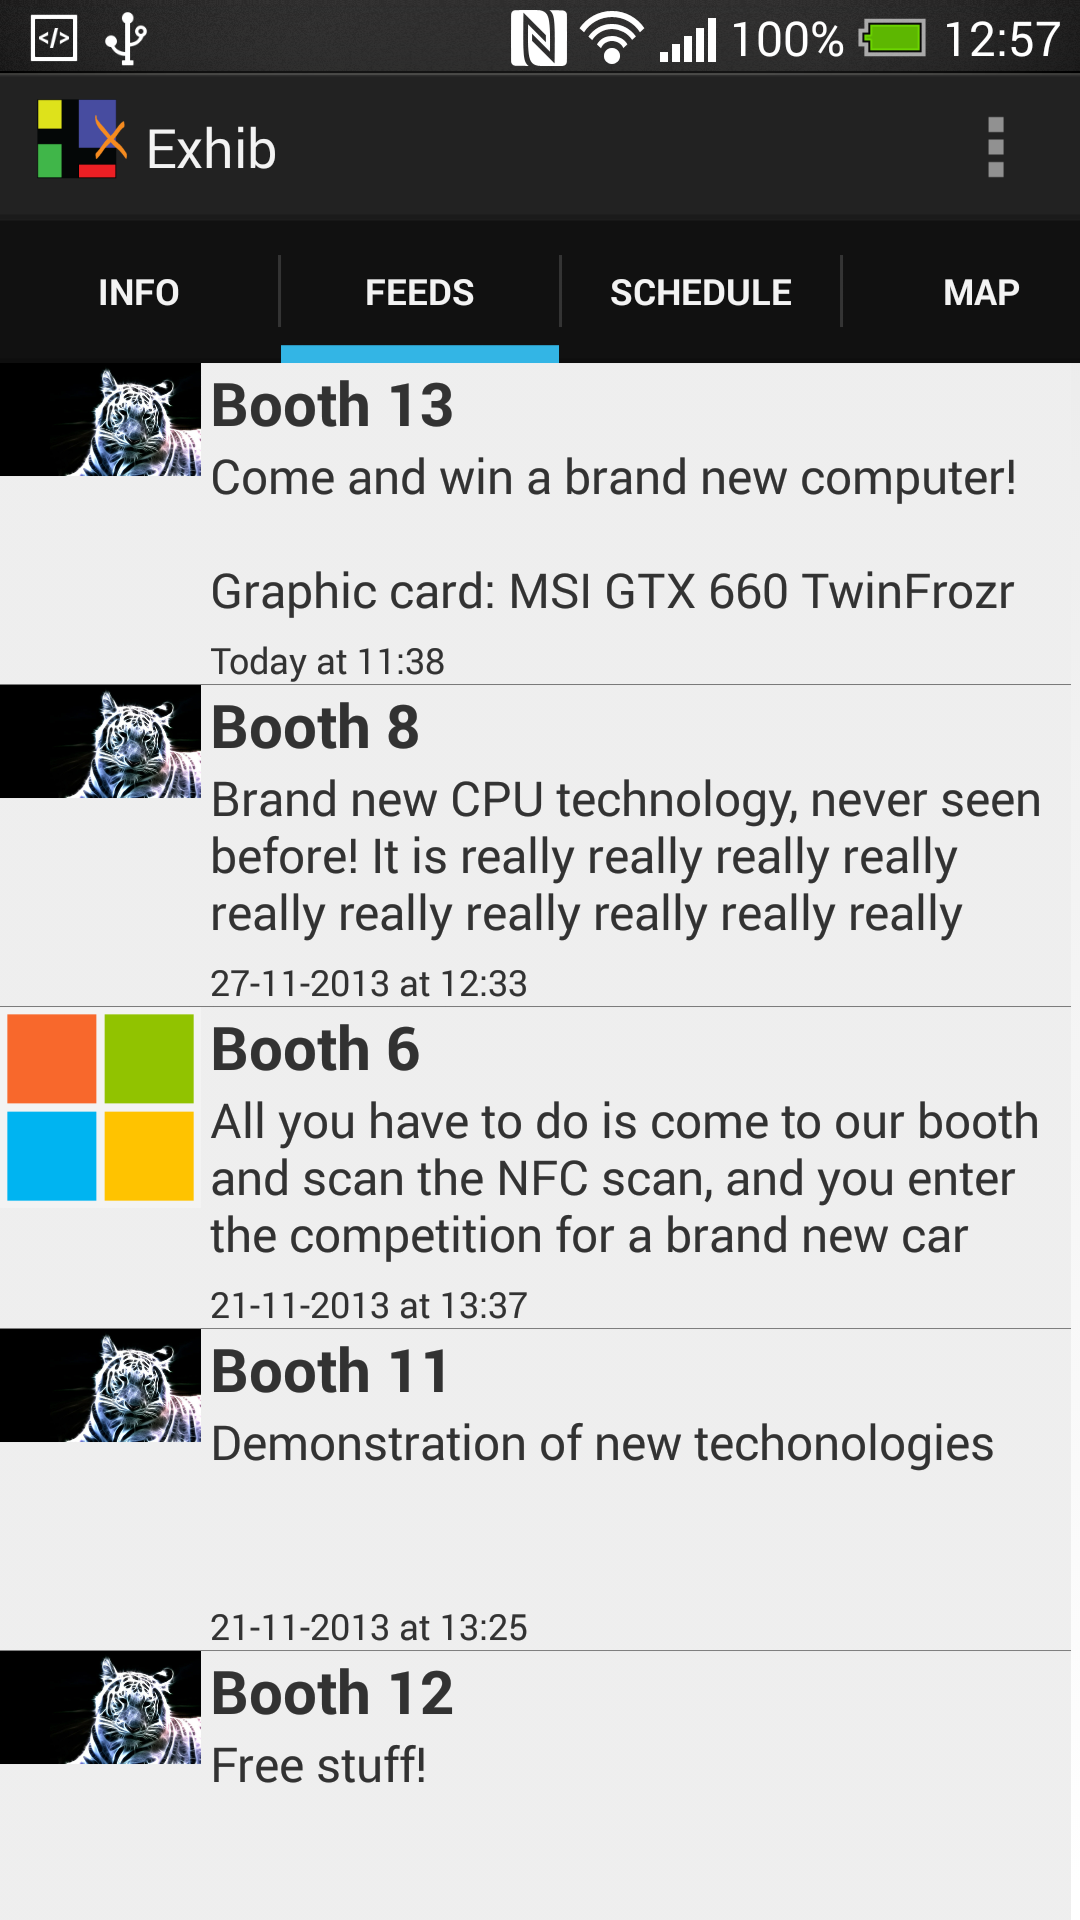
\includegraphics[width=0.7\columnwidth]{img/finaldesign/feedsscreen.png}
\caption{Feed list} 
\label{fig:feedsscreen}
\end{minipage}
\end{figure}

Some of the feeds are too long to display all the text in the list of feeds, so in order to read the full feed you can press the feed and a pop-up will come up displaying the full feed, as shown on \autoref{fig:popupfeed}. This is different from the prototype, because we thought it would be more convenient for the user to have a pop-up. During the exhibition, the booths might send new feeds, when this happens a button will be displayed, telling the user that more feeds are available, allowing them to choose when they want to load the new feeds so they always can make sure they have read all feeds before loading new ones. This can be seen on \autoref{fig:feedsnewitem}.

\begin{figure}[H]
\begin{minipage}[b]{0.5\columnwidth}
\centering
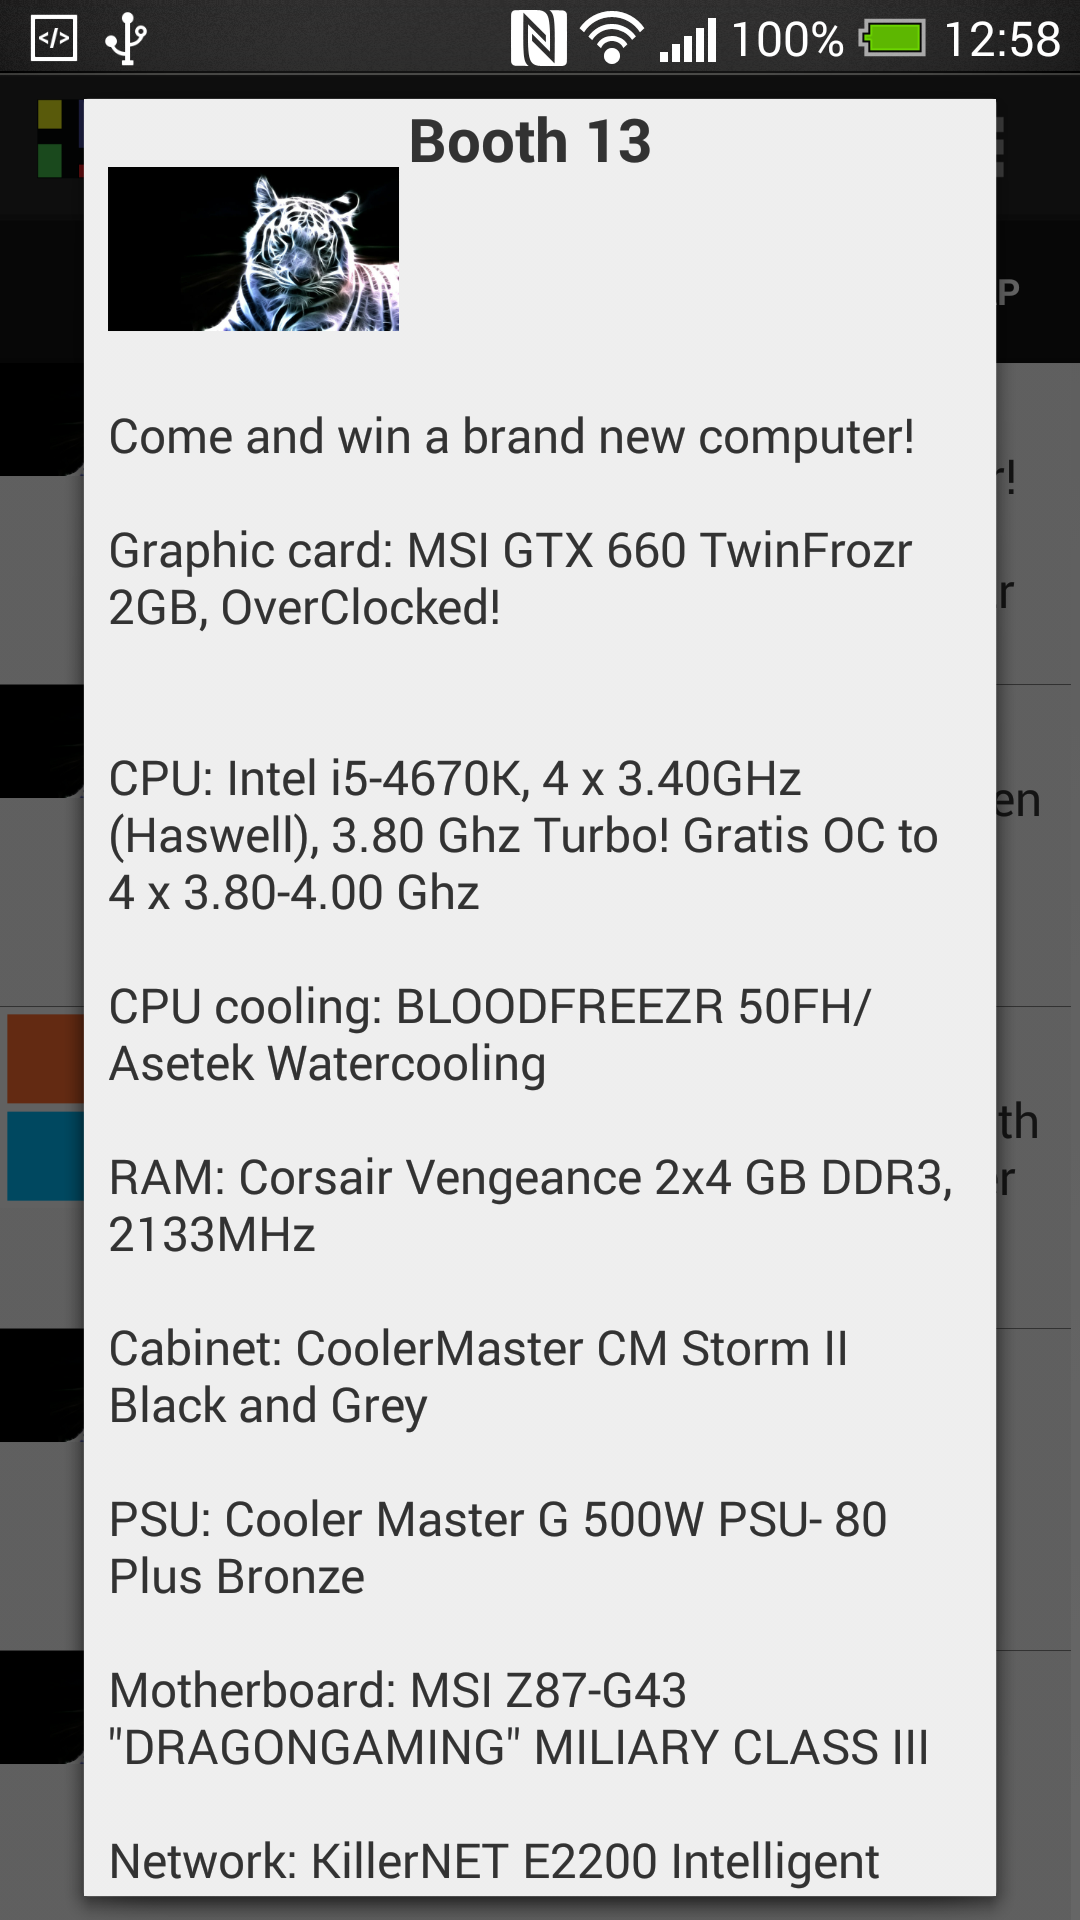
\includegraphics[width=0.7\columnwidth]{img/finaldesign/feedspopup.png}
\caption{Feed popup}
\label{fig:popupfeed}
\end{minipage}
\hspace{0.5cm}
\begin{minipage}[b]{0.5\columnwidth}
\centering
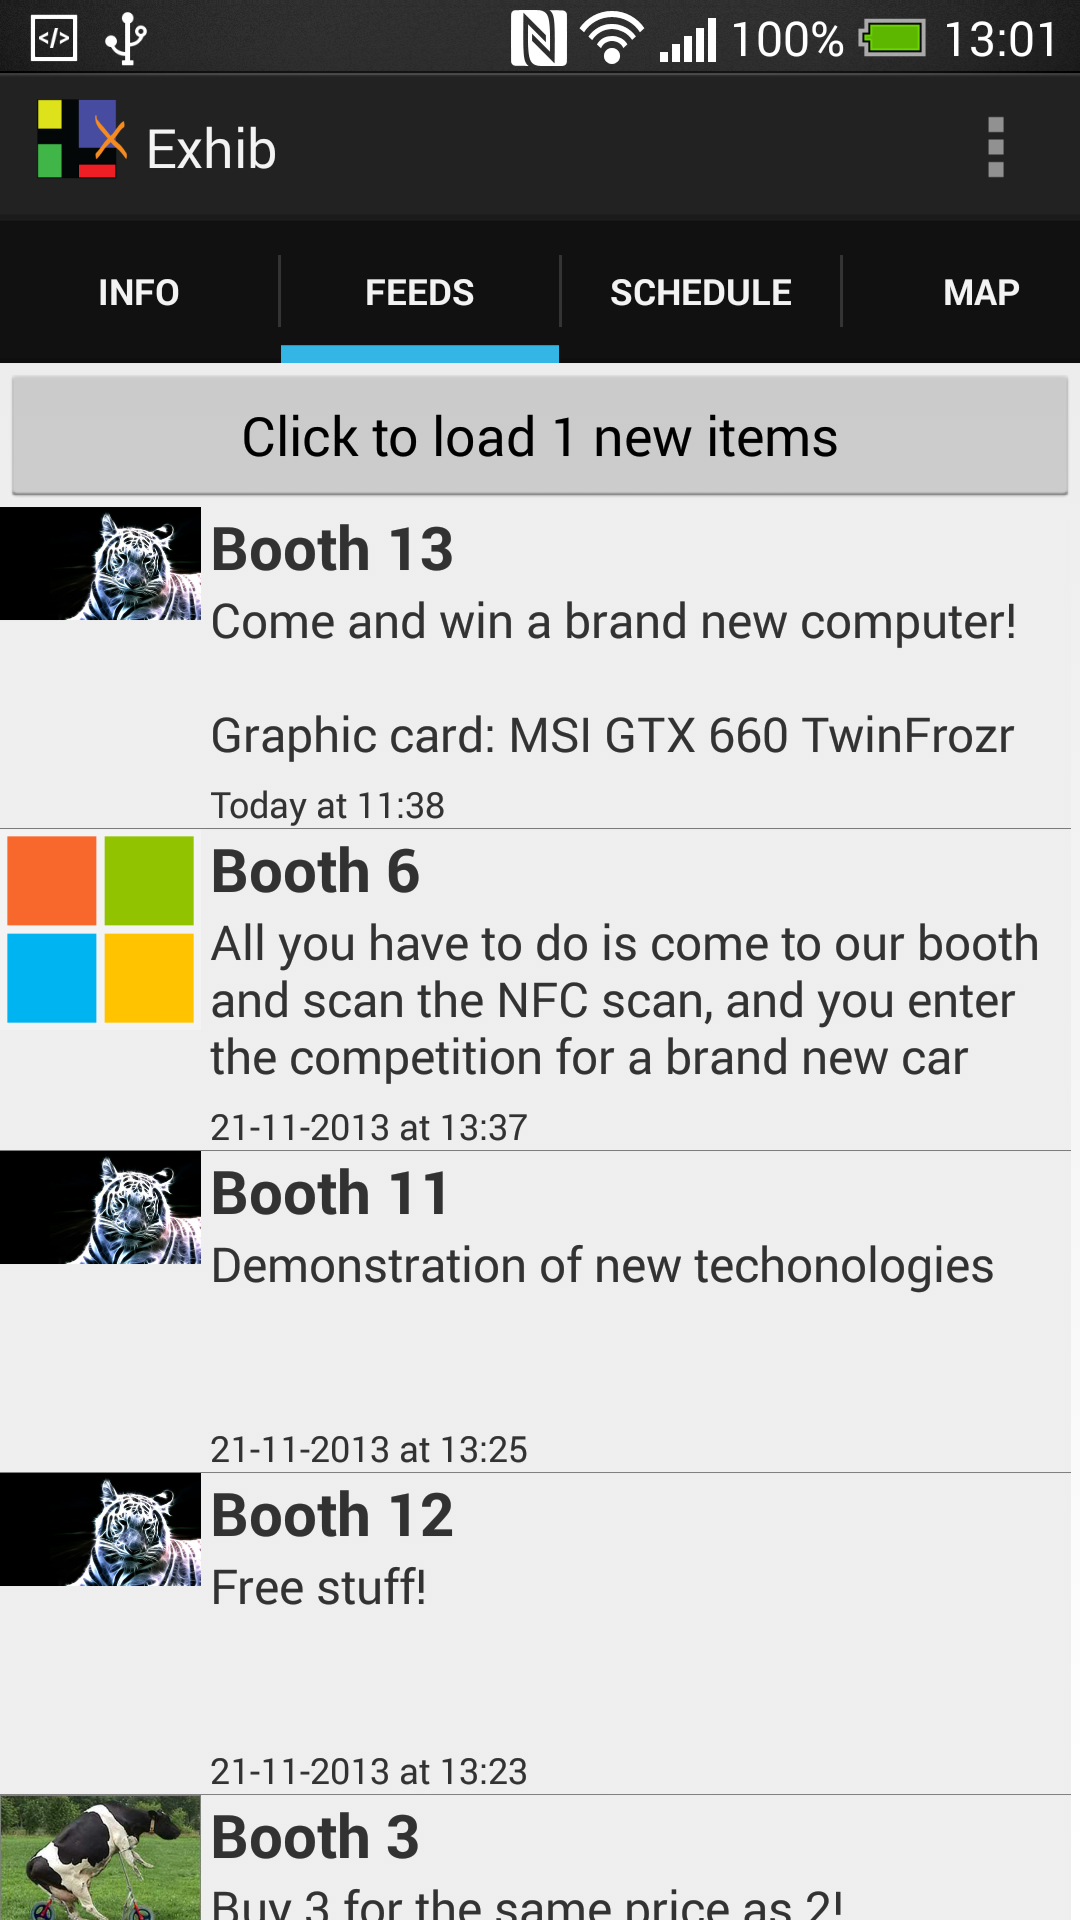
\includegraphics[width=0.7\columnwidth]{img/finaldesign/feedsnewitem.png}
\caption{New feed item}
\label{fig:feedsnewitem}
\end{minipage}
\end{figure}

The "Schedule" tab shows the events that is going on at the exhibition itself, could be a company presenting some new hardware or software at the main stage. This can be seen on \autoref{fig:schedule1}. Each event in the schedule has a countdown to when it will happen. 

The last tab is the map, this is a map over the exhibition, displaying all the booths on the exhibition. If you scan an \ac{nfc} on a booth the map will snap to that booth on the map and display a red circle to show where you are, this can be seen on \autoref{fig:map1}. You can also press the info icon on each booth, to receive information about this booth.

\begin{figure}[H]
\begin{minipage}[b]{0.5\columnwidth}
\centering
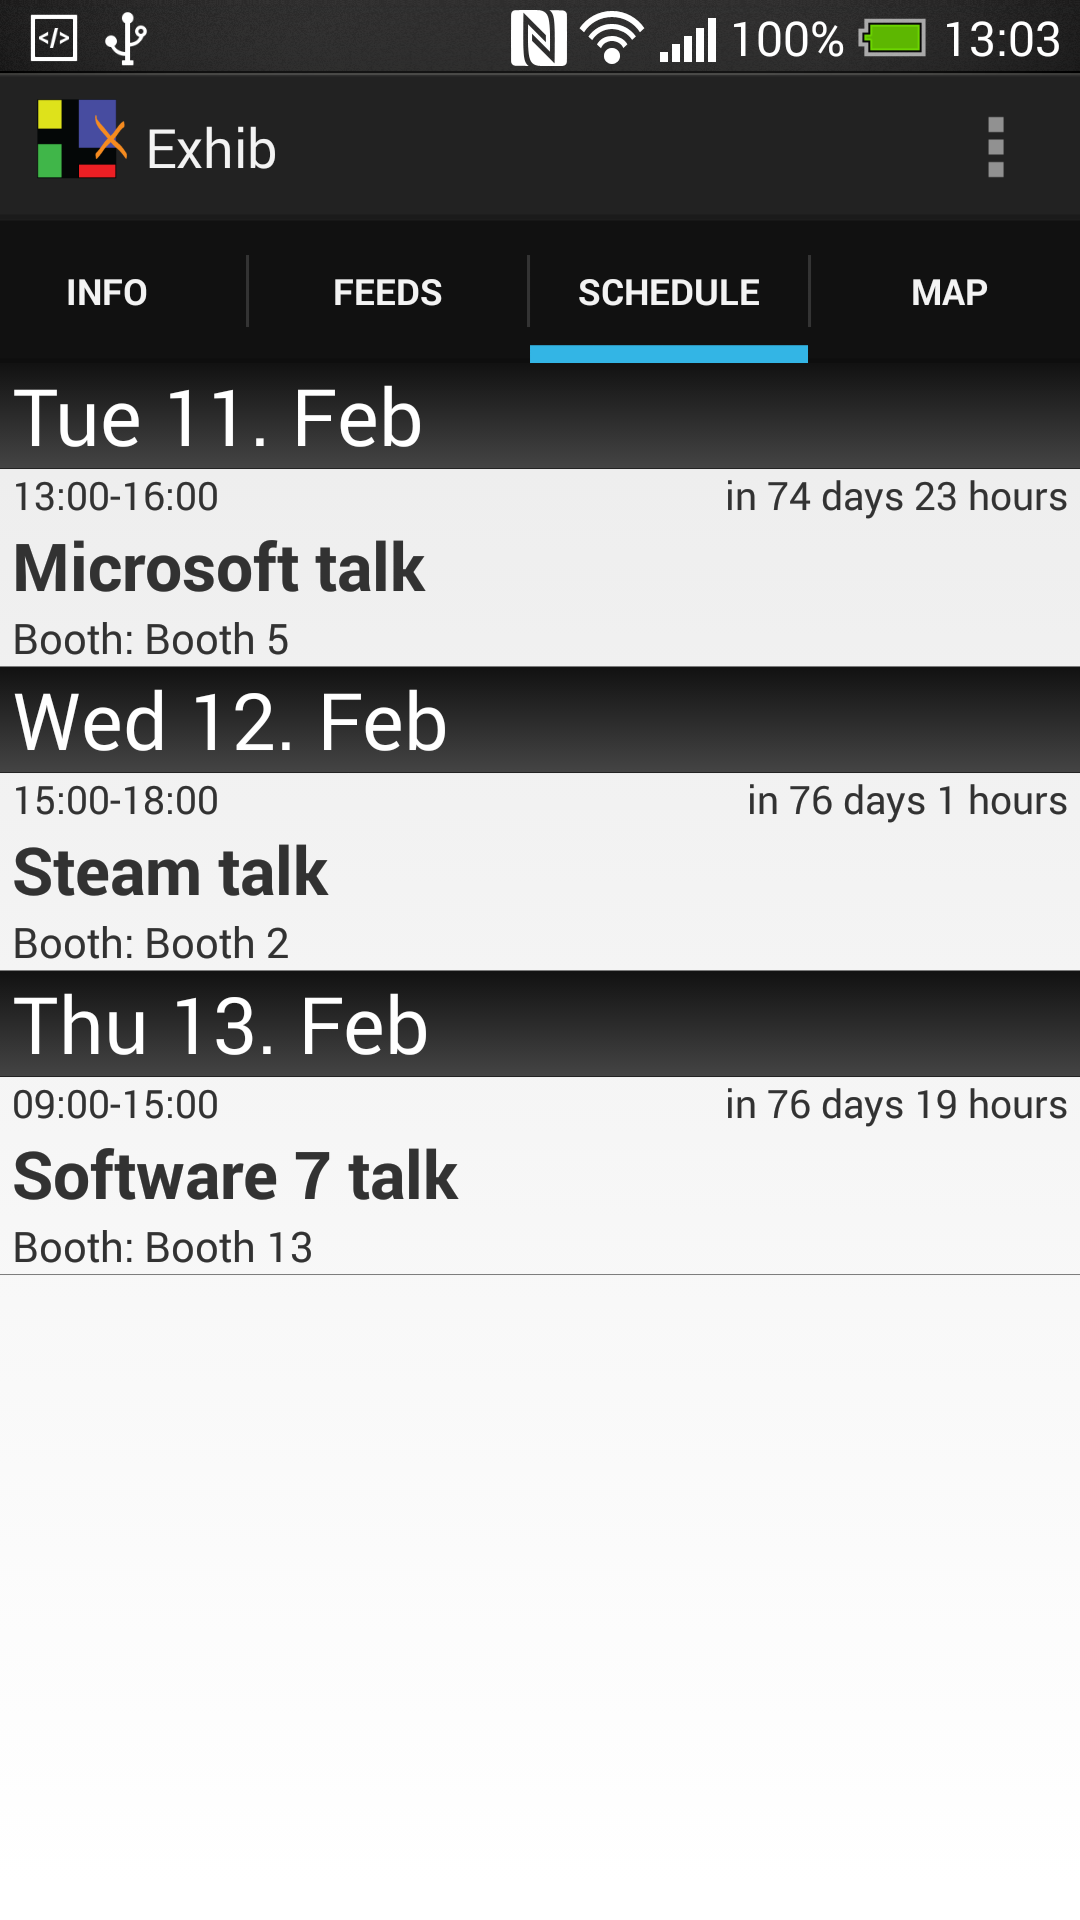
\includegraphics[width=0.7\columnwidth]{img/finaldesign/schedule.png}
\caption{Schedule}
\label{fig:schedule1}
\end{minipage}
\hspace{0.5cm}
\begin{minipage}[b]{0.5\columnwidth}
\centering
%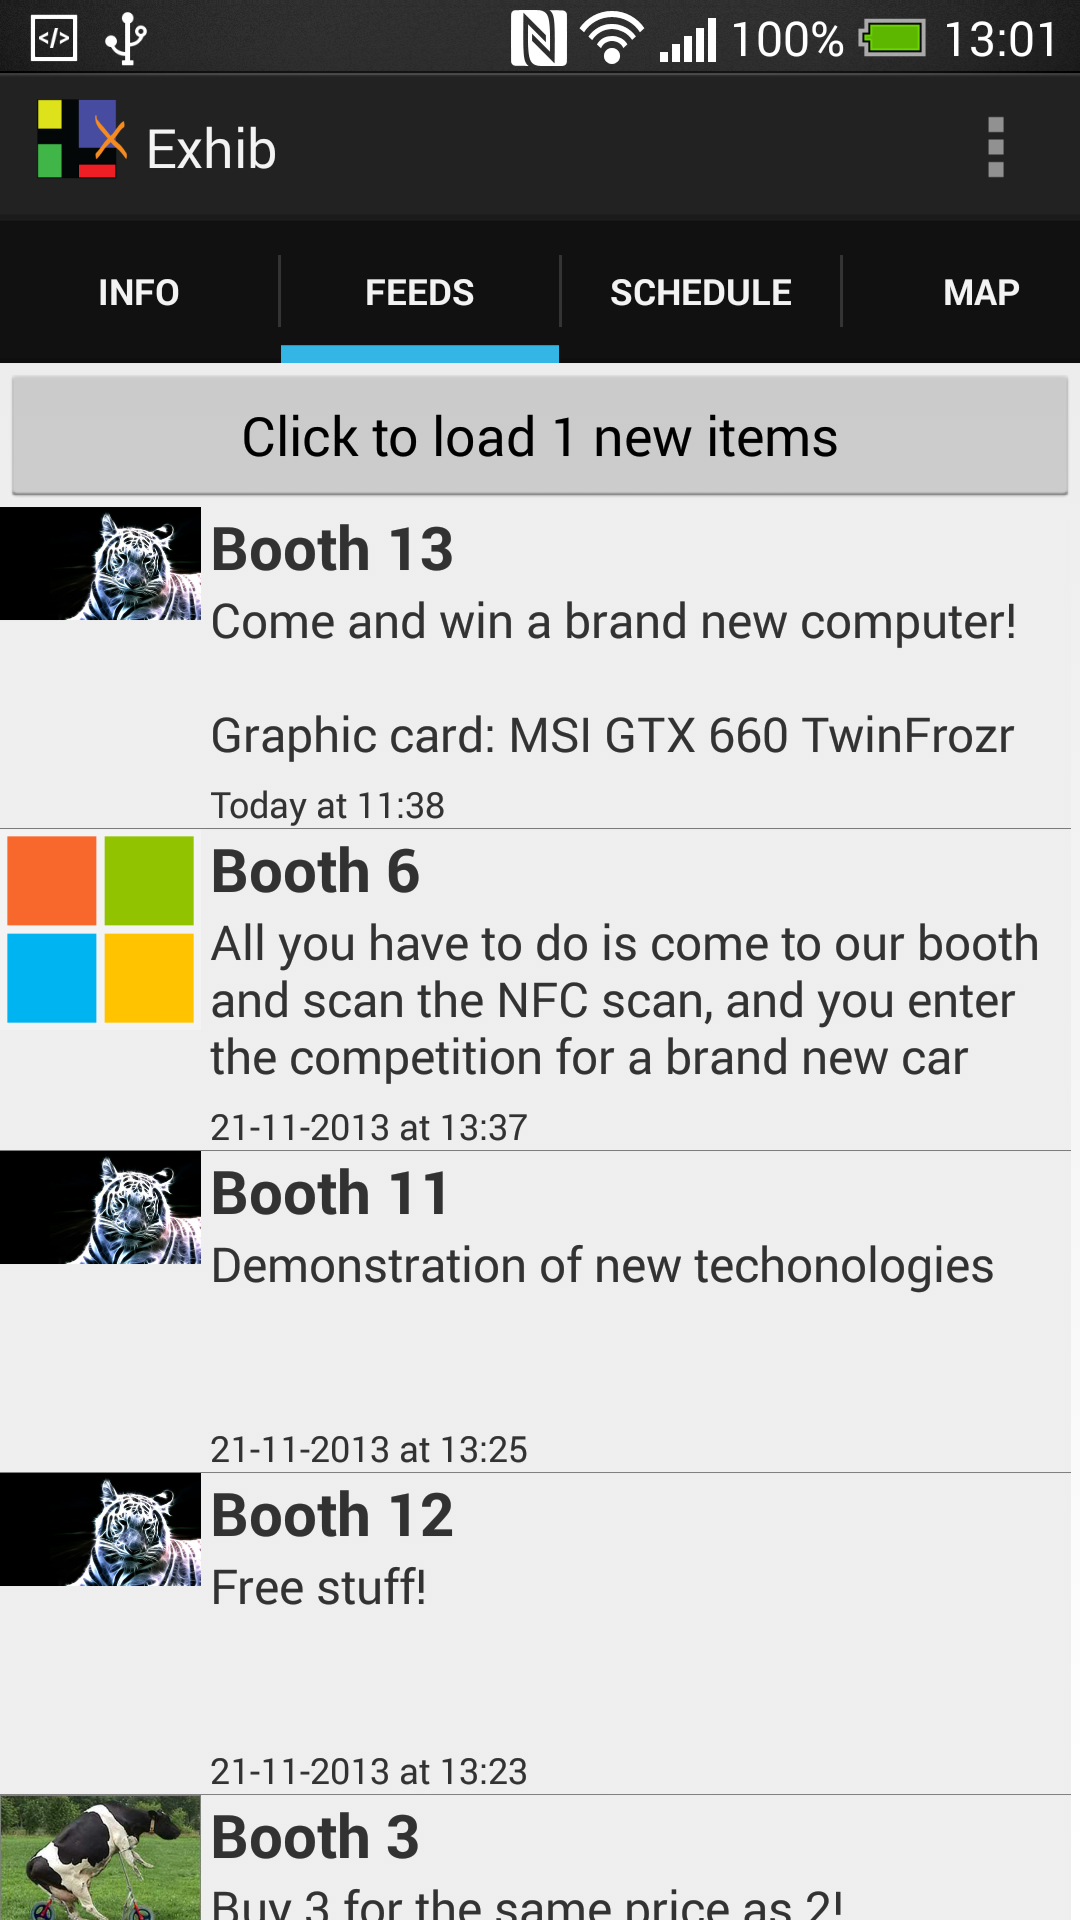
\includegraphics[width=0.7\columnwidth]{img/finaldesign/feedsnewitem.png}
\caption{Map}
\label{fig:map1}
%
\missingfigure{}
\end{minipage}
\end{figure}\todo{Picture of map goes here}

\autoref{fig:flowchart} show the application flow between these different activities. Note that the \textit{TabActivity} consists only of tabs, each tab is defined in a fragment.

\begin{figure}[H]
\centering
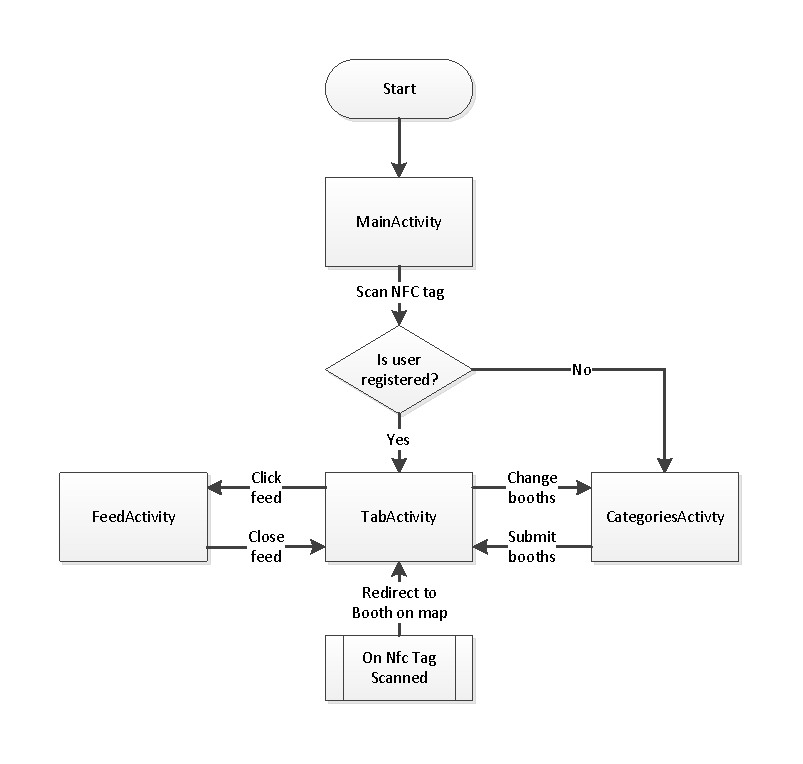
\includegraphics[width=\columnwidth]{img/appFlowchart.pdf}
\caption{Application actvity flow\label{fig:flowchart}}
\end{figure}
\todo{Pictures and description of the finished application}
